% This file was created with tikzplotlib v0.10.1.
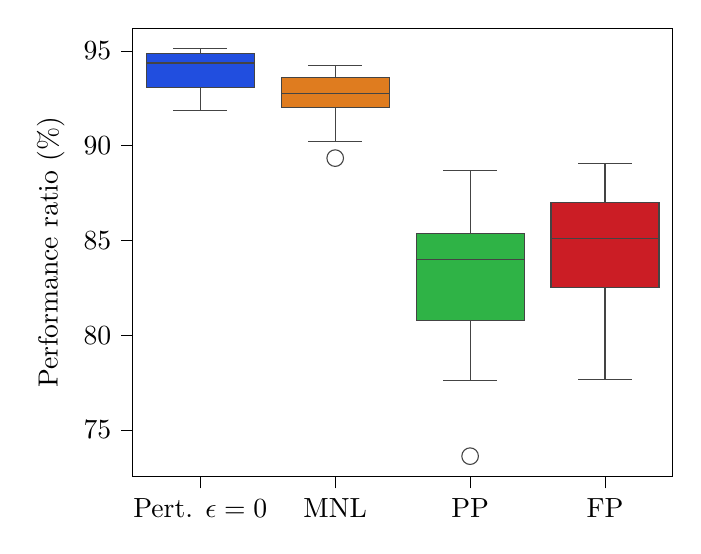
\begin{tikzpicture}

\definecolor{chocolate22312431}{RGB}{223,124,31}
\definecolor{darkgray176}{RGB}{176,176,176}
\definecolor{darkslategray68}{RGB}{68,68,68}
\definecolor{firebrick2032937}{RGB}{203,29,37}
\definecolor{limegreen4717970}{RGB}{47,179,70}
\definecolor{royalblue3378223}{RGB}{33,78,223}

\begin{axis}[
tick align=outside,
tick pos=left,
x grid style={darkgray176},
xmin=-0.5, xmax=3.5,
xtick style={color=black},
xtick={0,1,2,3},
xticklabels={Pert. \(\displaystyle \epsilon=0\),MNL,PP,FP},
y grid style={darkgray176},
ylabel={Performance ratio (\%)},
ymin=72.5467977566071, ymax=96.2003769214691,
ytick style={color=black},
ytick={70,75,80,85,90,95,100},
yticklabels={
  \(\displaystyle {70}\),
  \(\displaystyle {75}\),
  \(\displaystyle {80}\),
  \(\displaystyle {85}\),
  \(\displaystyle {90}\),
  \(\displaystyle {95}\),
  \(\displaystyle {100}\)
}
]
\path [draw=darkslategray68, fill=royalblue3378223]
(axis cs:-0.4,93.0765634615927)
--(axis cs:0.4,93.0765634615927)
--(axis cs:0.4,94.8837217605645)
--(axis cs:-0.4,94.8837217605645)
--(axis cs:-0.4,93.0765634615927)
--cycle;
\addplot [darkslategray68]
table {%
0 93.0765634615927
0 91.8523982442826
};
\addplot [darkslategray68]
table {%
0 94.8837217605645
0 95.1252142321572
};
\addplot [darkslategray68]
table {%
-0.2 91.8523982442826
0.2 91.8523982442826
};
\addplot [darkslategray68]
table {%
-0.2 95.1252142321572
0.2 95.1252142321572
};
\path [draw=darkslategray68, fill=chocolate22312431]
(axis cs:0.6,92.0224894960145)
--(axis cs:1.4,92.0224894960145)
--(axis cs:1.4,93.6162686656397)
--(axis cs:0.6,93.6162686656397)
--(axis cs:0.6,92.0224894960145)
--cycle;
\addplot [darkslategray68]
table {%
1 92.0224894960145
1 90.2346005578498
};
\addplot [darkslategray68]
table {%
1 93.6162686656397
1 94.2259197773107
};
\addplot [darkslategray68]
table {%
0.8 90.2346005578498
1.2 90.2346005578498
};
\addplot [darkslategray68]
table {%
0.8 94.2259197773107
1.2 94.2259197773107
};
\addplot [black, mark=o, mark size=3, mark options={solid,fill opacity=0,draw=darkslategray68}, only marks]
table {%
1 89.347001997502
};
\path [draw=darkslategray68, fill=limegreen4717970]
(axis cs:1.6,80.7656222923379)
--(axis cs:2.4,80.7656222923379)
--(axis cs:2.4,85.3874874430389)
--(axis cs:1.6,85.3874874430389)
--(axis cs:1.6,80.7656222923379)
--cycle;
\addplot [darkslategray68]
table {%
2 80.7656222923379
2 77.6341964522543
};
\addplot [darkslategray68]
table {%
2 85.3874874430389
2 88.7043764630758
};
\addplot [darkslategray68]
table {%
1.8 77.6341964522543
2.2 77.6341964522543
};
\addplot [darkslategray68]
table {%
1.8 88.7043764630758
2.2 88.7043764630758
};
\addplot [black, mark=o, mark size=3, mark options={solid,fill opacity=0,draw=darkslategray68}, only marks]
table {%
2 73.621960445919
};
\path [draw=darkslategray68, fill=firebrick2032937]
(axis cs:2.6,82.5021621714283)
--(axis cs:3.4,82.5021621714283)
--(axis cs:3.4,87.0227157031759)
--(axis cs:2.6,87.0227157031759)
--(axis cs:2.6,82.5021621714283)
--cycle;
\addplot [darkslategray68]
table {%
3 82.5021621714283
3 77.6603881814643
};
\addplot [darkslategray68]
table {%
3 87.0227157031759
3 89.0406873356241
};
\addplot [darkslategray68]
table {%
2.8 77.6603881814643
3.2 77.6603881814643
};
\addplot [darkslategray68]
table {%
2.8 89.0406873356241
3.2 89.0406873356241
};
\addplot [darkslategray68]
table {%
-0.4 94.3656415323535
0.4 94.3656415323535
};
\addplot [darkslategray68]
table {%
0.6 92.7418460931945
1.4 92.7418460931945
};
\addplot [darkslategray68]
table {%
1.6 84.0058825970647
2.4 84.0058825970647
};
\addplot [darkslategray68]
table {%
2.6 85.0975996089361
3.4 85.0975996089361
};
\draw (axis cs:0,66.6334029653916) node[
  scale=0.75,
  anchor=base,
  text=black,
  rotate=0.0
]{\bfseries 94.00};
\draw (axis cs:1,66.6334029653916) node[
  scale=0.75,
  anchor=base,
  text=black,
  rotate=0.0
]{\bfseries 92.61};
\draw (axis cs:2,66.6334029653916) node[
  scale=0.75,
  anchor=base,
  text=black,
  rotate=0.0
]{\bfseries 83.05};
\draw (axis cs:3,66.6334029653916) node[
  scale=0.75,
  anchor=base,
  text=black,
  rotate=0.0
]{\bfseries 84.65};
\draw (axis cs:-1,66.8699387570403) node[
  scale=0.75,
  text=black,
  rotate=0.0
]{\bfseries \textbf{Average:}};
\end{axis}

\end{tikzpicture}
